%%%%%%%%%%%%%%%%%%%%%%%%%%%%%%%%%%%%%%%%%
% Journal Article
% LaTeX Template
% Version 1.3 (9/9/13)
%
% This template has been downloaded from:
% http://www.LaTeXTemplates.com
%
% Original author:
% Frits Wenneker (http://www.howtotex.com)
%
% License:
% CC BY-NC-SA 3.0 (http://creativecommons.org/licenses/by-nc-sa/3.0/)
%
%%%%%%%%%%%%%%%%%%%%%%%%%%%%%%%%%%%%%%%%%

%----------------------------------------------------------------------------------------
%	PACKAGES AND OTHER DOCUMENT CONFIGURATIONS
%----------------------------------------------------------------------------------------

\documentclass[twoside]{article}

\usepackage{lipsum} % Package to generate dummy text throughout this template

\usepackage[sc]{mathpazo} % Use the Palatino font
\usepackage[T1]{fontenc} % Use 8-bit encoding that has 256 glyphs
\linespread{1.05} % Line spacing - Palatino needs more space between lines
\usepackage{microtype} % Slightly tweak font spacing for aesthetics
\usepackage{alltt}

\usepackage[hmarginratio=1:1,top=32mm,columnsep=20pt]{geometry} % Document margins
\usepackage{multicol} % Used for the two-column layout of the document
\usepackage[hang, small,labelfont=bf,up,textfont=it,up]{caption} % Custom captions under/above floats in tables or figures
\usepackage{booktabs} % Horizontal rules in tables
\usepackage{float} % Required for tables and figures in the multi-column environment - they need to be placed in specific locations with the [H] (e.g. \begin{table}[H])
\usepackage{hyperref} % For hyperlinks in the PDF

\usepackage{lettrine} % The lettrine is the first enlarged letter at the beginning of the text
\usepackage{paralist} % Used for the compactitem environment which makes bullet points with less space between them

\usepackage{abstract} % Allows abstract customization
\renewcommand{\abstractnamefont}{\normalfont\bfseries} % Set the "Abstract" text to bold
\renewcommand{\abstracttextfont}{\normalfont\small\itshape} % Set the abstract itself to small italic text
\usepackage{graphicx}

\usepackage{titlesec} % Allows customization of titles
\renewcommand\thesection{\Roman{section}} % Roman numerals for the sections
\renewcommand\thesubsection{\Roman{subsection}} % Roman numerals for subsections
\titleformat{\section}[block]{\large\scshape\centering}{\thesection.}{1em}{} % Change the look of the section titles
\titleformat{\subsection}[block]{\large}{\thesubsection.}{1em}{} % Change the look of the section titles

\usepackage{fancyhdr} % Headers and footers
\pagestyle{fancy} % All pages have headers and footers
\fancyhead{} % Blank out the default header
\fancyfoot{} % Blank out the default footer
\fancyhead[C]{Getting started with OpenRISC on the SocKit} % Custom header text
\fancyfoot[RO,LE]{\thepage} % Custom footer text

\newcommand{\M}{$\rightarrow$}

%----------------------------------------------------------------------------------------
%	TITLE SECTION
%----------------------------------------------------------------------------------------

\title{\vspace{-15mm}\fontsize{24pt}{10pt}\selectfont\textbf{Getting
    started with OpenRISC on the SocKit}} % Article title

\author{
\large
\textsc{Hans Baier}\thanks{Thanks to Stefan Kristiansson for his
  generous help and Kevin Mehall for his excellent tutorial on the de0\_nano}\\[2mm] 
\normalsize \href{mailto:hansfbaier@gmail.com}{hansfbaier@gmail.com} % Your email address
\vspace{-5mm}
}
\date{}

%----------------------------------------------------------------------------------------

\begin{document}

\maketitle % Insert title

\thispagestyle{fancy} % All pages have headers and footers

%----------------------------------------------------------------------------------------
%	ABSTRACT
%----------------------------------------------------------------------------------------

\begin{abstract}

  \noindent Getting started with OpenRISC can be quite daunting for
  beginners. There is so much to learn. Fortunately the community is
  very helpful. In order to diminish duplication of effort, this
  tutorial was conceived out of the generous hours of support that
  Stefan Kristiansson provided over IRC. This tutorial also provides
  some of the supplemental files, for convenience.

\end{abstract}

%----------------------------------------------------------------------------------------
%	ARTICLE CONTENTS
%----------------------------------------------------------------------------------------

%\begin{multicols}{2} % Two-column layout throughout the main article text

\section{Introduction}

\lettrine[nindent=0em,lines=3]{O} penRISC is an amazing learning
plattform: You can run Open Source Software on Open Source Hardware
and see down to the metal, how hardware is designed, drivers are
written, and how software and hardware interact.  

%------------------------------------------------

\section{Prerequisites}
This tutorial assumes you are using a GNU/Linux Distribution. This
tutorial is based on Ubuntu 12.04 (precise).

\begin{compactitem}
\item Experience with Linux systems
\item Compiling software from source
\item Basic understanding of digital logic, communication protocols
  and electronics.
\item Familiarity with Verilog and C
\end{compactitem}

You will need a Linux workstation with a 64 Bit operating system, 8GB
of RAM and about 20-30GB free hard drive space. You will also need
terasic's
\href{http://www.terasic.com.tw/cgi-bin/page/archive.pl?Language=English\&No=816}{SocKit
  Development Board}.

%------------------------------------------------

\section{Step By Step}
\begin{enumerate}
\item Install \href{http://dl.altera.com/?edition=web}{Altera Quartus
    II Web Edition} at least version 13.0sp1. For this tutorial we assume
  you installed it in \texttt{/opt/altera/}

\item Download the
  \href{http://www.terasic.com.tw/cgi-bin/page/archive.pl?Language=English\&CategoryNo=165\&No=816\&PartNo=4}{resources}
  for the development board. Find out what board revision you have
  (first PDF on the resources page), and download the SocKit System CD
  for the correct board revision. This will be most likely be Revision
  C at the time of this writing:
  \begin{alltt}
\$ wget -c http://www.terasic.com/downloads/cd-rom/sockit/SoCKit\_V.1.0.0\_System.zip
  \end{alltt}

\item Install development tools:
  \begin{alltt}
\$ sudo apt-get install build-essential libmpc-dev libgmp3-dev libmpfr-dev  \textbackslash
                       lzop libsdl1.2-dev xterm automake libtool \textbackslash
                       git-core git subversion iverilog device-tree-compiler
  \end{alltt}

\item Create the directory where we put openrisc related files:
  \begin{alltt}
\$ mkdir ~/openrisc
  \end{alltt}

\item Create a file with necessary environment variables:
  \begin{alltt}
\$ cd ~/openrisc
\$ editor altera_env.sh
\hrulefill
export ALTERA_PATH=/opt/altera
export PATH=$PATH:$ALTERA_PATH/quartus/bin
\hrulefill
\$ source altera_env.sh
  \end{alltt}
  You may want to source this file every time you want to use Altera's
  tools.

\item Unpack the SocKit CD:
  \begin{alltt}
\$ mkdir CD
\$ unzip ../SoCKit\_V.1.0.0\_System.zip -d CD
  \end{alltt}

\item Get \texttt{orpsoc} which is the OpenRISC-SoC-Builder and
  \texttt{orpsoc-cores}, which contains the IP-cores and board
  configurations:
  \begin{alltt}
\$ git clone https://github.com/openrisc/orpsoc.git
\$ git clone https://github.com/skristiansson/orpsoc-cores.git
  \end{alltt}

\item Build and install OrpSoC:
  \begin{alltt}
\$ cd orpsoc
\$ autoreconf -i && ./configure && make && sudo make install
  \end{alltt}

\item Configure orpsoc-cores and test:
  \begin{alltt}
\$ cd ../orpsoc-cores/
\$ editor orpsoc.conf
\hrulefill
[main]
cores_root   = ./cores
systems_root = ./systems
\hrulefill
\$ orpsoc sim wb_bfm
Preparing wb_bfm
Preparing vlog_tb_utils
All tests passed!
  \end{alltt}

\item We need to start a first run on building the sockit. It will
  fail, because the Qsys infrastructure Verilog files don't exist yet.
  We need this run, though, since the target directory for the Qsys
  files does not exist yet:
  \begin{alltt}
\$ orpsoc build sockit    
  \end{alltt}

\item We now need to generate the infrastructure Verilog files for the
  HPS system. Fire up Quartus:
  \begin{alltt}
\$ quartus &
  \end{alltt}

\item Close the splash screen and start Qsys with: Tools\M Qsys

\item Open Qsys file with: File\M Open

\item Choose File: \texttt{systems/sockit/data/sockit.qsys}

\item Klick on the 'Generation' Tab and choose for Output Directory
  (relative to orpsoc-cores): \texttt{build/sockit/src/qsys/}

  This takes a while. Get a glass of orange juice (healthier than
  coffee) or do a couple of pushups in the meantime.

\item When Generation is finished successfully, close the dialog, save
  the Qsys (then the output path will be right when you choose to
  alter the Qsys and need to rerun again).

\item Close Qsys and Quartus and
  build the FPGA bitstream:
  \begin{alltt}
\$ orpsoc build sockit    
  \end{alltt}

  Once more, this takes quite a while, depending on your machine. Time
  for another glass of orange juice and some pushups.

  If all went well, then you should have the file
  \texttt{build/sockit/bld-quartus/sockit.sof}. This is the bitstream
  for the FPGA:
  \begin{alltt}
\$ find . | grep sof\$
./build/sockit/bld-quartus/sockit.sof    
  \end{alltt}

\item If you are done with the pushups, and it is still compiling, you
  can continue with the following steps until you need the Bitstream
  (\texttt{.sof}).

\item Download the
  \href{http://dl.altera.com/?edition=web#tabs-2}{Altera Embedded
    Design Suite} (DS-5) Web Edition. Select the tab 'Individual
  Files' and klick the Download link for the Embedded Design Suite.

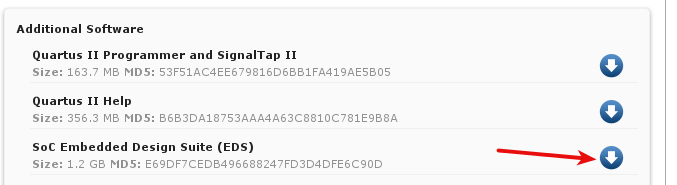
\includegraphics[width=\textwidth]{download-eds.png}

\item Install it to \texttt{/opt/altera/} as well. If everything went
  right, you should have a subdirectory
  \texttt{/opt/altera/embedded/}. This is the installation location of
  the embedded design suite.

\item Setup you SocKit Board. The Clock and Bootsel Jumpers need to
  look like this:

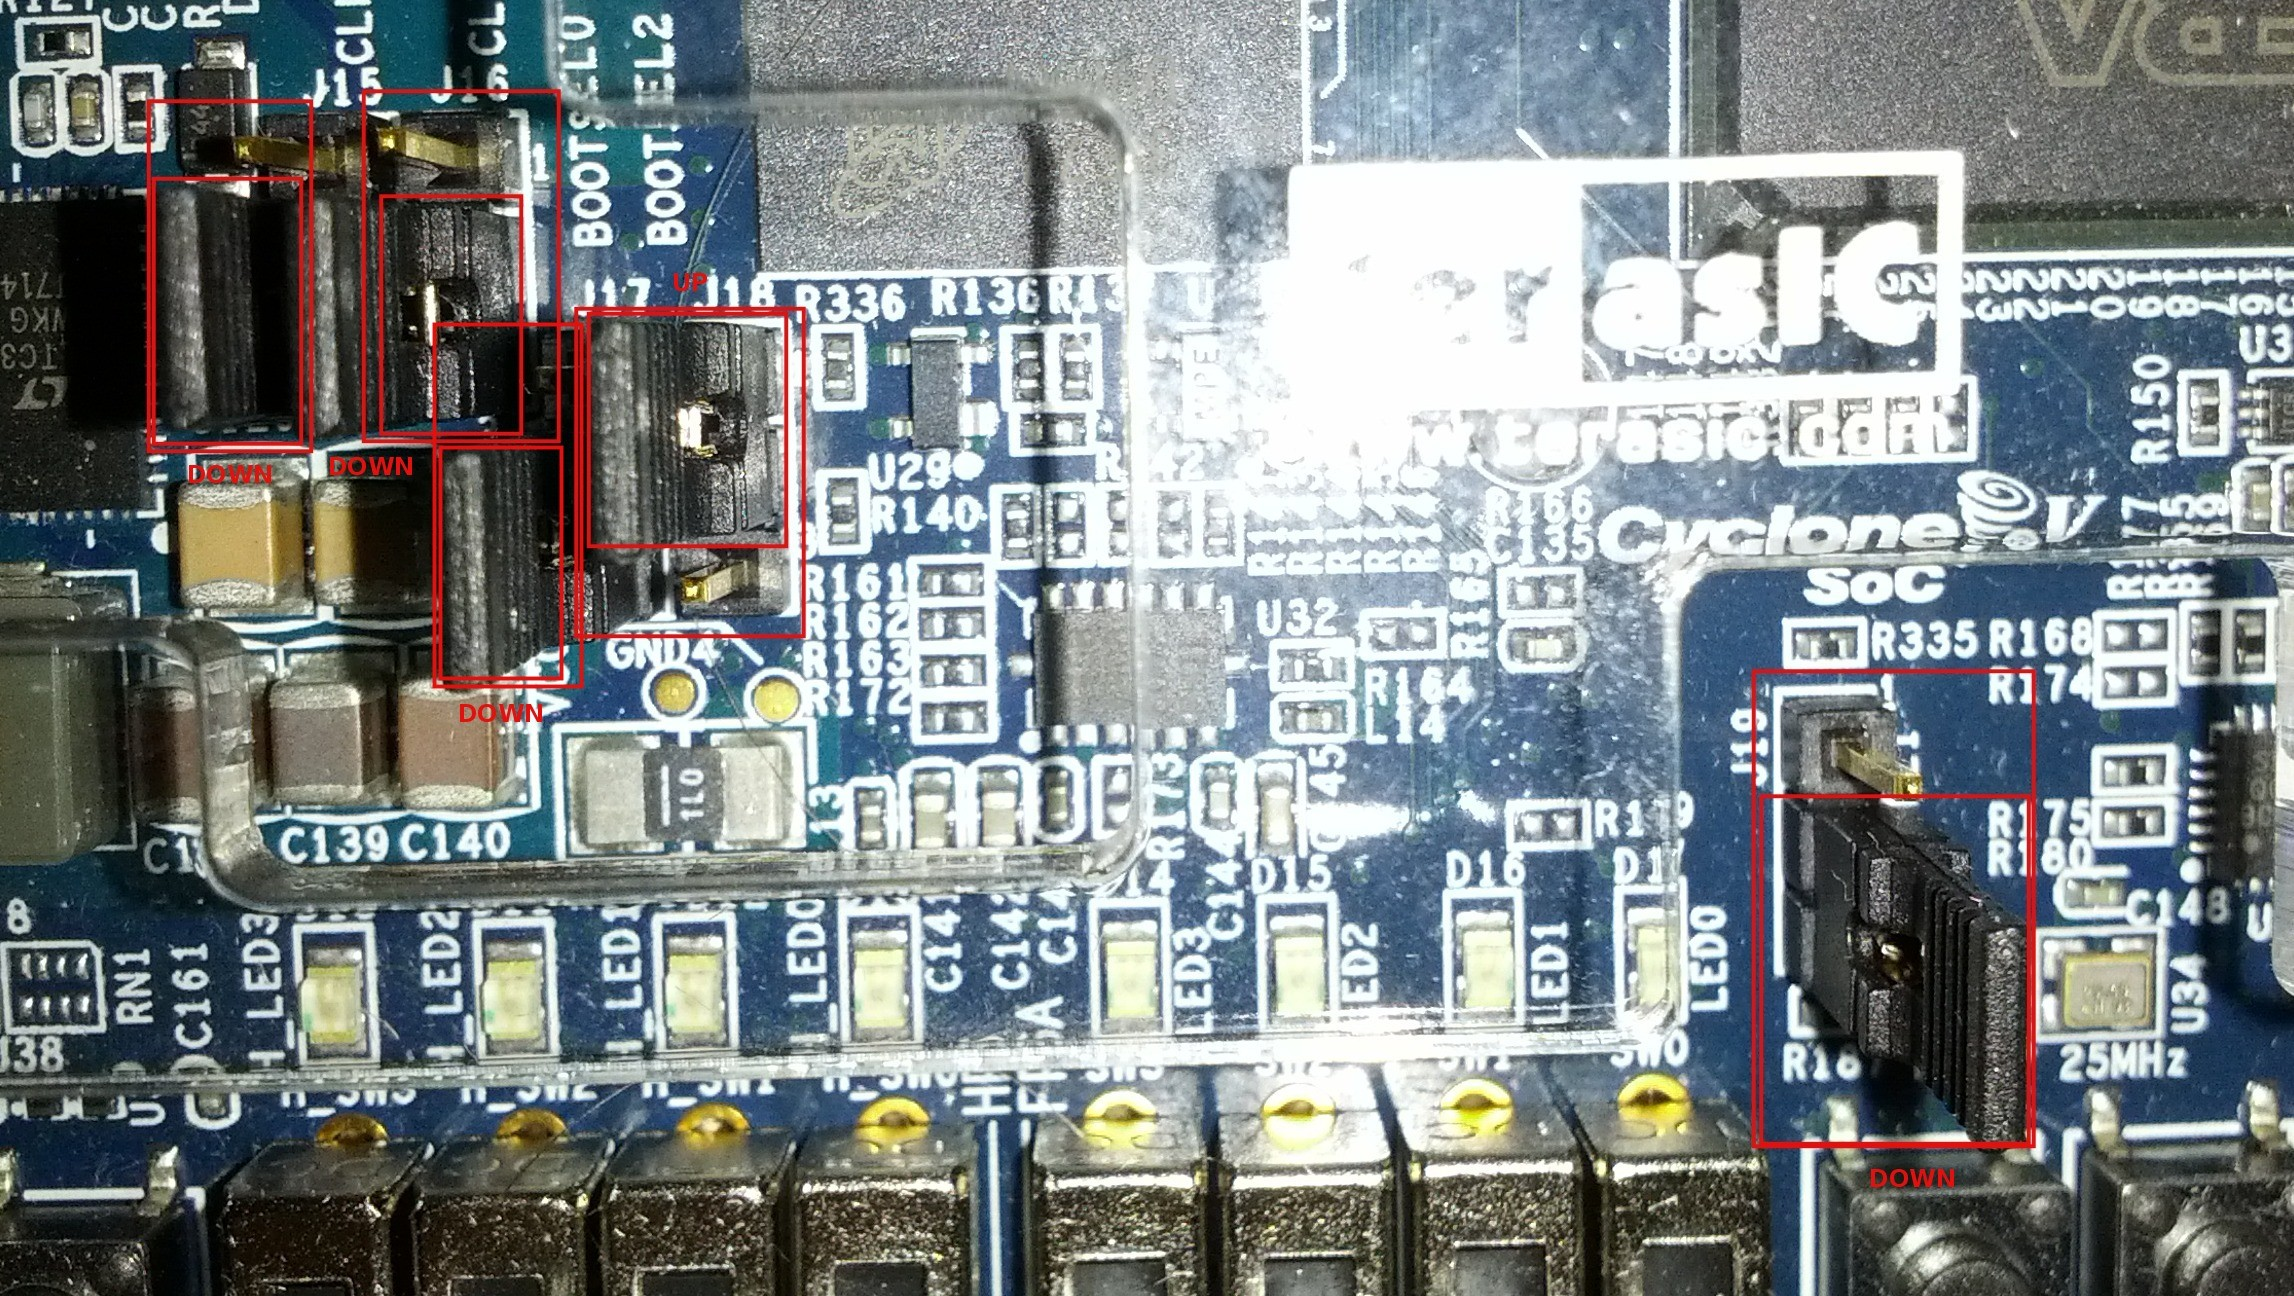
\includegraphics[width=0.8\textwidth]{boardjumpers.jpeg}

\item In order to boot Linux from the ARM-HPS, the MSEL dipswitch has
  to be set to passive serial (10000) like this:

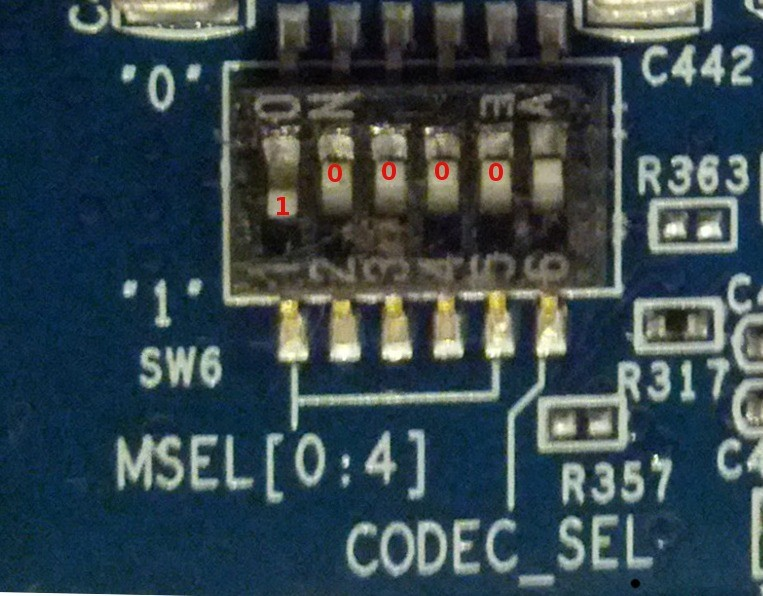
\includegraphics[width=0.6\textwidth]{dipswitch.jpeg}

Note that '0' on the board corresponds to 'ON' on the
DIP-switch. Trust the board, not the switch. The last DIP-switch is
probably irrelevant, I didn't bother to find out, you can let it how
it came in the box. Don't blame me if your board catches fire or
kills your cat.

\item The JTAG-DIP-switch should be set to bypass the HSMC connector
  and to enable the HPS. (That's '01' in the orientation of the silk
  screen print):

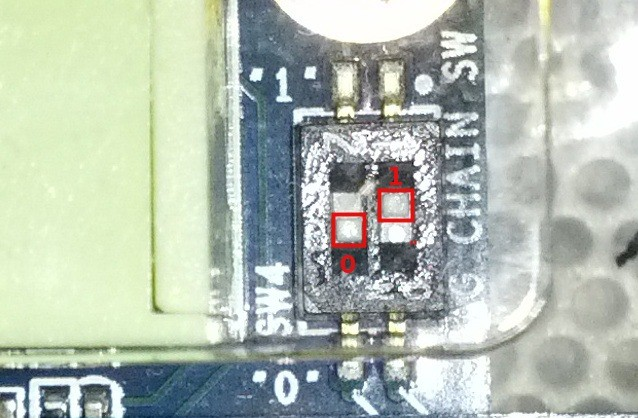
\includegraphics[width=0.5\textwidth]{jtagswitch.jpeg}

\item Make sure the USB Blaster II integrated on the board has proper
  permissions. 
  \begin{alltt}
\$ editor /etc/udev/rules.d/81-usbblaster.rules   
\hrulefill
# USB-Blaster II
SUBSYSTEM=="usb", ATTRS{idVendor}=="09fb", ATTRS{idProduct}=="6010", MODE="0666"
SUBSYSTEM=="usb", ATTRS{idVendor}=="09fb", ATTRS{idProduct}=="6810", MODE="0666"
\hrulefill
  \end{alltt}

  I had to put two versions of the \texttt{idProduct} into the file,
  since the product id mutated since first plug in. If in doubt, check
  your Blaster with \texttt{lsusb} and alter \texttt{idProduct}
  accordingly.

\item Start the Altera embedded command shell:
  \begin{alltt}
\$ /opt/altera/embedded/embedded_command_shell.sh
  \end{alltt}

\item Start the BSP-Editor to create a board support package for the
  Qsys generated platform;
  \begin{alltt}
\$ bsp-editor   
  \end{alltt}

\item Klick Menu: File\M New BSP

\item For 'Preloader settings directory' choose

  \texttt{orpsoc-cores/build/sockit/bld-quartus/hps\_isw\_handoff/sockit\_hps\_0}

\item Press 'OK'

\item Press 'Generate'

\item Press 'Exit' if everything went well during generation.

\item Go to the generated sources and build them:
  \begin{alltt}
\$ cd orpsoc-cores/build/sockit/bld-quartus/software/spl_bsp/    
\$ make
  \end{alltt}
  This will extract the \texttt{uboot} source code into the
  subdirectory \texttt{uboot-socfpga}.

\item Now if everything went well, we need to modify uboot, so that
  the wishbone system on the FPGA is reset automatically on boot time:
  \begin{alltt}
\$ editor uboot-socfpga/include/configs/socfpga_cyclone5.h
\hrulefill
    "mmcboot=\underline{mw 0xffd0501c 4;}setenv bootargs " CONFIG_BOOTARGS \textbackslash
\hrulefill
  \end{alltt}

\item Rebuild:
  \begin{alltt}
\$ make all    
  \end{alltt}

\item Then you are ready to prepare the SD card. You need an SD card
  large enough (2GB) to accomodate the Factory image. We extract the
  factory from on the SocKit CD and write it on SD card. Please note,
  that \texttt{/dev/sd\emph{X}} denotes the device of your sd card.

  \begin{alltt}
\$ cd ~/openrisc/CD/Tools/Factory_SD_image/
\$ unrar x SoCKit_SD.rar 
\$ sudo dd if=SoCKit_SD.img of=/dev/sd\emph{X} bs=512
\$ sudo sync
\$ sudo eject /dev/sd\emph{X}
  \end{alltt}

\item The layout should contain three partitions like this:
  \begin{alltt}
\$ sudo fdisk -l /dev/sd\emph{X}

   Device Boot      Start         End      Blocks   Id  System
/dev/sdX1         2121728     2162687       20480    b  W95 FAT32
/dev/sdX2           14336     2111487     1048576   83  Linux
/dev/sdX3            2048        4095        1024   a2  Unknown    
  \end{alltt}
Note there is one FAT-Partition. This one contains the device tree and
the uboot kernel image (\texttt{uImage}). The second partition
(Linux) contains the Linux root filesystem. The third partition (type
\texttt{a2}) contains the bootloader and uboot. It has no filesystem
on it.

\item Before we modify the SD card, you might want to verify it boots
  (without our openrisc FPGA image flashed). 
  To do this, 
  \begin{enumerate}
  \item connect the USB serial cable to your Host PC 
  \item Insert the SD card into the SoCKit
  \item Power the board on
  \item Fire up a terminal
    program of your choice on the virtual USB terminal (we assume
    \texttt{/dev/ttyUSB0}):
    \begin{alltt}
\$ picocom /dev/ttyUSB0 -b 57600
    \end{alltt}
    You might want to use \texttt{sudo} here if you don't have an
    appropriate \texttt{udev} entry or you are not a member of the
    \texttt{dialout} group.
    Do this quickly after the board is powered on to catch as much of
    the boot messages as possible.
  \end{enumerate}

  It should boot uboot and then Linux. If that is the case, you are
  fine for now. If not, you have a problem\dots

\item If Linux boots fine, switch off the device (we will replace the
  Linux system on it)

\item We will replace the Yocto Linux system with a Debian system
  (optional, but needed for convenient software install):
  \begin{alltt}
\$ wget -c
http://www.rocketboards.org/pub/Projects/Debian/debian.img.gz
\$ gunzip debian.img.gz
\$ sudo dd if=debian.img of=/dev/sd\emph{X}2 bs=512
  \end{alltt}

You can also use an ubuntu based image, like Stefan:
\begin{scriptsize}
  \begin{alltt}
\$ wget -c \textbackslash
https://releases.linaro.org/13.04/ubuntu/quantal-images/developer/linaro-quantal-developer-20130422-342.tar.gz
  \end{alltt}
\end{scriptsize}
but this image is unsupported (by me) since I did not try it.

\item Next thing is to build the Linux kernel for the ARM based HPS system:
  \begin{alltt}
\$ cd ~/openrisc
\$ mkdir sockit
\$ mv CD sockit
\$ cd sockit
\$ git clone --depth 1 git://git.rocketboards.org/linux-socfpga.git 
\$ cd linux-socfpga
\$ 
  \end{alltt}
\end{enumerate}

%----------------------------------------------------------------------------------------
%	REFERENCE LIST
%----------------------------------------------------------------------------------------

\begin{thebibliography}{99} 

\bibitem[rocketboards]{rocketboards:2013} \url{www.rocketboards.org}
  Resource website for SoCKit and related boards. Lots of useful
  information and software.

\end{thebibliography}

%----------------------------------------------------------------------------------------

%\end{multicols}

\end{document}